\documentclass{article}
\usepackage[utf8]{inputenc}
\usepackage{graphicx}

\title{Project for CTA200H}
\author{Ming Liang Ang}
\date{May 2022}

\begin{document}

\maketitle

\section{Question 2}
\subsection{Question 2.3: How does the radial velocity curve depend on each of these?}
As the mass of the star increases, the period decreases and the magnitude of the radial velocity oscillation decreases and vice versa. 
\begin{figure}[!h]
    \begin{center}
    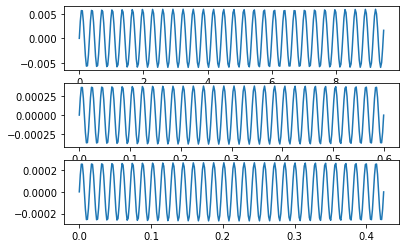
\includegraphics[scale=0.5]{mass_star.png}
    \end{center}
  \caption{RV plot when the mass of the star changes}
\end{figure}
\\\\
As the mass of the planet increases, the period decreases and the magnitude of the radial velocity oscillation increases and vice versa
\begin{figure}[!h]
    \begin{center}
    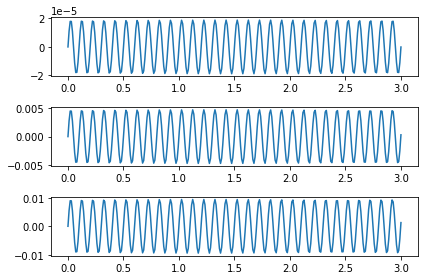
\includegraphics[scale=0.4]{mass_planet.png}
    \end{center}
  \caption{RV plot when the mass of the orbiting planet changes}
\end{figure}
\\\\
As the semi major axis of the planet increases, the period decreases and the magnitude of the radial velocity oscillation decreases. 
\begin{figure}[h!]
\begin{center}
    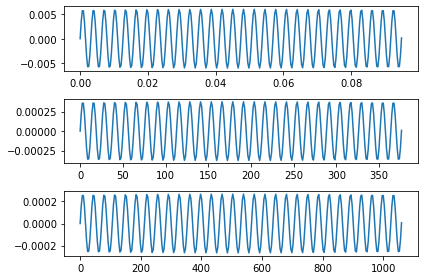
\includegraphics[scale=0.4]{semi_major_axis.png}
    \end{center}
  \caption{RV plot when the semi major axis of the orbiting planet changes}
\end{figure}
\newpage
\subsection{Question 2.4: What changes when $e=0.3$?}
The RV curve is no longer a plane wave. The peaks also oscillate.
\begin{figure}[!h]
    \begin{center}
    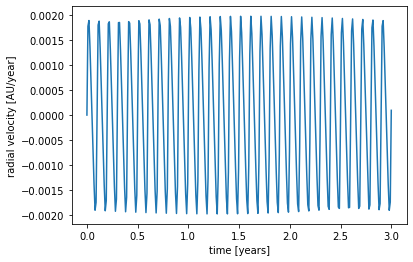
\includegraphics[scale=0.5]{e_0.3.png}
    \end{center}
  \caption{RV plot when e-0.3}
\end{figure}
\newpage
\newpage
\section{Question 3}
\subsection{Question 2.5.5: Are the values similar to those which RS2017 found?}
The values found are similar (within the error bar) of what RS2017 found. 
\subsection{Question 2.5.6: The values with errors?}
The estimated error bars are:\\\\
\noindent
$m_1$:  $ 0.941839713 \pm 1.29144185 \times 10^{-2}$\\
$m_2$: $ 0.869533382 \pm 1.30311416\times 10^{-2}$$\\
$a_1$: $0.658420910\pm 8.79431067\times 10^{-3}$\\
$a_2$: $1.04188007 \pm 1.33763092 \times 10^{-2}$\\
$M_1$: $93.2194881 \pm 1.56581118$\
$M_2$: $182.084202 \pm 2.71507998$\\
$h_1$: $0.153473237 \pm 1.81059100\times 10^{-3}$\\
$h_2$: $8.05361883 \times 10^{-2}\pm 1.01197608 \times 10^{-3}$\\
$k_1$: $-8.34870780 \times 10^{-2}\pm 1.14976032 \times 10^{-3}$\\
$k_2$: $-6.32399766 \times 10^{-2} \pm 9.87196198 \times 10^{-4}$\\
$\gamma$: $3.8568885 \pm 5.29191840 \times 10^{-2}$\\
$\sigma_j$: $2.95393147 \pm 3.88170120\times 10^{-2}$
\subsection{Question 2.5.7: Does the fit look good?}
The fit does not look good, compared to the fit from the paper. 
\\\\
\begin{figure}[!h]
    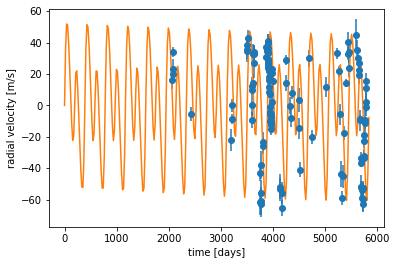
\includegraphics[scale=0.5]{output.png}
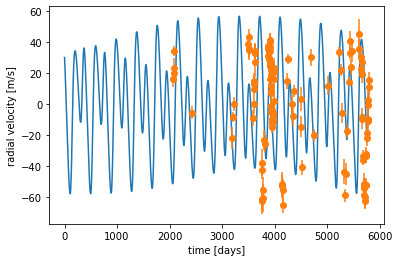
\includegraphics[scale=0.5]{output2.png}
  \caption{Left: Parameters from  RS2017 Right: Parameters from  emcee}
\end{figure}
\end{document}
